\documentclass[xcolor=table,10pt,aspectratio=169]{beamer}

\usepackage[l2tabu,orthodox]{nag}

\usepackage[english]{babel}

\usepackage{microtype}
\usepackage{graphicx}
\usepackage{color}
\usepackage{enumitem}
\usepackage[normalem]{ulem}

\newlist{todolist}{itemize}{2}
\setlist[todolist]{label=$\square$}

\usepackage{float}
\usepackage{array}
\usepackage{tabularx}
\newcolumntype{L}[1]{>{\raggedright\arraybackslash}p{#1}}
\newcolumntype{C}[1]{>{\centering\arraybackslash}p{#1}}
\newcolumntype{R}[1]{>{\raggedleft\arraybackslash}p{#1}}
\usepackage{booktabs}
\usepackage{subcaption}
\usepackage{cancel}

% multiline comment
\newcommand{\comment}[1]{}

% convert to roman
\newcommand{\Rnum}[1]{\uppercase\expandafter{\romannumeral #1\relax}}
\newcommand{\rnum}[1]{\lowercase\expandafter{\romannumeral #1\relax}}

% cryptobib
\usepackage[
    advantage,
    adversary,
    asymptotics,
    complexity,
    events,
    ff,
    % keys,
    lambda,
    landau,
    logic,
    mm,
    notions,
    operators,
    oracles,
    primitives,
    probability,
    sets]{cryptocode}

\renewcommand{\pcthen}{\highlightkeyword{\,:\ }}
\renewcommand{\pcelse}{\highlightkeyword{else:\ }}
\newcommand{\pcbreak}{\highlightkeyword{break}}

\usepackage{amssymb}
\let\proof\relax\let\endproof\relax
\usepackage{amsthm}
\usepackage{amsfonts}
\usepackage{xspace}

%\usepackage[bookmarksdepth=2,pagebackref=true,breaklinks=true]{hyperref}
%\hypersetup{
%    colorlinks,
%    linkcolor={black},
%    citecolor={black},
%    urlcolor={blue!80!black},
%}

\usepackage{ifdraft}

\ifdraft{
    \NewDocumentCommand \ben  {s m o} {\IfBooleanTF{#1}{\cmnt*{ben}{#2}}{\cmnt{ben}{#2}[#3]}}
}{
    \NewDocumentCommand\ben  {s m o} {}
}

%% LISTINGS

\usepackage[final]{listings}
\lstdefinelanguage{Sage}[]{Python}{morekeywords={True,False,sage,cdef,cpdef,ctypedef,self},sensitive=true}

\lstset{frame=none,
  showtabs=False,
  showspaces=False,
  showstringspaces=False,
  commentstyle={\color{gray}},
  keywordstyle={\color{black}\textbf},
  stringstyle={\color{darkgray}},
  basicstyle=\tt\scriptsize\relax,
  inputencoding=utf8, literate={…}{{\ldots}}1{λ}{{\(\lambda\)}}1{ε}{{\(\varepsilon\)}}1{σ}{{\(\sigma\)}}1{⋅}{{\(\cdot\)}}1{κ}{{\(\kappa\)}}1{‖}{{\(\Vert\)}}1{γ}{{\(\gamma\)}}1{≤}{{\(\leq\)}}1{β}{{\(\beta\)}}1{η}{{\(\eta\)}}1{×}{{\(\times\)}}1,
  belowskip=0.0em,}


\usepackage[color={.9 .2 .2},final]{attachfile2}


%%% Local Variables:
%%% mode: LaTeX
%%% TeX-master: "lip"
%%% End:


% sets
\newcommand{\ter}{\ensuremath{\set{-1,0,1}}}
% matrix groups
\newcommand{\GL}{\mathcal{GL}}
\newcommand{\SL}{\mathcal{SL}}
\newcommand{\Ort}{\mathcal{O}}
\newcommand{\QF}{\mathcal{S}^{>0}}
% \newcommand{\HF}{\mathcal{H}^{>0}}
% relations
\newcommand{\from}{\leftarrow}
\newcommand{\idtfy}{\longleftrightarrow}
\newcommand{\into}{\hookrightarrow}
\newcommand{\iso}{\cong}
% algebra
\DeclareMathOperator{\HNF}{HNF}
\DeclareMathOperator{\SF}{SF}
\DeclareMathOperator{\QR}{QR}
\DeclareMathOperator{\Hom}{Hom}
\DeclareMathOperator{\Tor}{Tor}
\DeclareMathOperator{\Ext}{Ext}
\DeclareMathOperator{\Aut}{Aut}
\DeclareMathOperator{\End}{End}
\DeclareMathOperator{\Gal}{Gal}
\DeclareMathOperator{\Span}{Span}
\DeclareMathOperator{\diag}{diag}
\DeclareMathOperator{\rank}{rank}
\DeclareMathOperator{\hull}{hull}
\DeclareMathOperator{\codim}{codim}
\DeclareMathOperator{\tr}{tr}
\DeclareMathOperator{\GF}{GF}
\DeclareMathOperator{\Spec}{Spec}
\DeclareMathOperator{\mSpec}{mSpec}
% algebraic numbers
\newcommand{\ring}{\ensuremath{\mathcal{R}}}
\newcommand{\field}{\ensuremath{\mathcal{K}}}
\newcommand{\lattice}{\ensuremath{\mathcal{L}}}
\newcommand{\variety}{\ensuremath{\mathcal{V}}}
% distributions
\newcommand{\unif}[1]{\ensuremath{\mathcal{U}\left( #1 \right)}}
% codes
\newcommand{\code}{\ensuremath{\mathfrak{C}}}
% crypto
\newcommand{\upd}{\ensuremath{\mathsf{Upd}}}
\newcommand{\updpk}{\ensuremath{\mathsf{UpdPk}}}
\newcommand{\updsk}{\ensuremath{\mathsf{UpdSk}}}
\newcommand{\game}{\ensuremath{\mathsf{Game}}}
\newcommand{\up}{\ensuremath{\mathsf{up}}}
\newcommand{\queries}{\ensuremath{\mathcal{Q}}\xspace}
\newcommand{\MsgSp}{\ensuremath\mathcal{M}}
\newcommand{\msg}{\ensuremath\mathsf{msg}}
\newcommand{\ctxt}{\ensuremath\mathsf{ctxt}}
\newcommand{\pk}{\ensuremath\mathsf{pk}}
\newcommand{\sk}{\ensuremath\mathsf{sk}}
\newcommand{\state}{\ensuremath\mathsf{st}}
% problems
\newcommand{\LWE}{\ensuremath{\text{LWE}}}
\newcommand{\RLWE}{\ensuremath{\text{MLWE}}}
\newcommand{\MLWE}{\ensuremath{\text{MLWE}}}
\newcommand{\SIS}{\ensuremath{\text{SIS}}}
\newcommand{\DSIS}{\ensuremath{\text{DSIS}}}
\newcommand{\PCE}{\ensuremath{\text{PCE}}}
\newcommand{\SPCE}{\ensuremath{\text{SPCE}}}
\newcommand{\LCE}{\ensuremath{\text{LCE}}}

% matrices and vectors
\renewcommand{\vec}[1]{\ensuremath{\mathbf{#1}}\xspace}
\newcommand{\mat}[1]{\ensuremath{\mathbf{#1}}\xspace}
\newcommand{\inner}[2]{\ensuremath{\langle #1, #2 \rangle}}
\newcommand{\transpose}{\mathtt{T}}

% notation
\newcommand{\algo}[1]{\ensuremath{\mathsf{#1}}\xspace}
\newcommand{\rnd}{\rho}
% \newcommand{\norm}[1]{\ensuremath{\lvert\lvert #1 \rvert\rvert}}
% \newcommand{\floor}[1]{\ensuremath{\left\lfloor #1 \right\rfloor}}
% \newcommand{\ceil}[1]{\ensuremath{\left\lceil #1 \right\rceil}}
\newcommand{\round}[1]{\ensuremath{\left\lfloor #1 \right\rceil}}

\newcommand{\SampleSelfOrthogonal}{\algo{SSO}}
\newcommand{\EnumSelfOrthogonal}{\algo{EnumSelfOrthogonal}}
\newcommand{\SampleCode}{\algo{SampCode}}
\newcommand{\SampleUnifCode}{\algo{SampleUnifCode}}
\newcommand{\SampleCodeShort}{\algo{SampleCodeShort}}

\mathchardef\mhyphen="2D


\usepackage{presentation}

\graphicspath{ {./pictures/} }

\usepackage{tikzpeople}
\usepackage{drawmatrix}

\def\isnonexpert{1}
\if\isnonexpert1
    \NewDocumentCommand \nonexpert {+m +m} {#1}
\else
    \NewDocumentCommand \nonexpert {+m +m} {#2}
\fi

\title{Hollow LWE: A New Spin --- Unbounded Updatable Encryption from LWE and PCE}
\author{\underline{Martin~R.~Albrecht}\thanks{Slides heavily based on Benjamin's slides.} (King's College London and SanboxAQ), Benjamin~Ben{\v c}ina (Royal Holloway, University of London) and Russell~W.~F.~Lai (Aalto University)}
\date{Workshop On the Mathematics of Post-Quantum Cryptography, Zürich, 6 June 2025}

\begin{document}

\titlepage

\begin{frame}{Public-Key Encryption (PKE)}
  \begin{figure}
    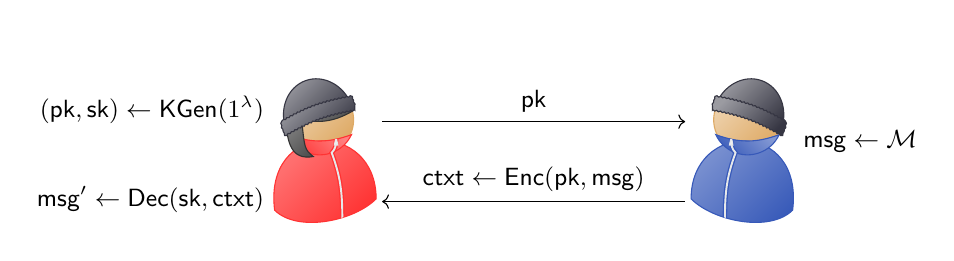
\begin{tikzpicture}[font=\small]
      \node (title) {};
      \node[criminal,female,shirt=red,minimum size=1.3cm, anchor=north west] at ($(title.south east)+(0,-.5)$) (A) {};
      \node[criminal,right=4cm of A,minimum size=1.3cm,mirrored] (B) {};
      \node[anchor=north east] at (A.north west) (a1)  {$(\pk, \sk) \gets \kgen(\secparam)$};
      \draw (A.35) edge[->] node[above] {$\pk$} (B.145);
      \node[anchor=south west] at (B.east |- B.180) {$\msg \gets \MsgSp$};
      \draw (A.-35) edge[<-] node[above] {$\ctxt \gets \enc(\pk, \msg)$} (B.215);
      \node[anchor=south east] at (A.south west) (a2)  {$\msg' \gets \dec(\sk, \ctxt)$};
    \end{tikzpicture}
  \end{figure}
  \vfill
  Properties:
  \begin{itemize}[label=\textbullet]
    \item Decryption Correctness: \(\msg' = \msg\).
    \item IND-CPA Security:
      \[
        \big(\pk, \enc(\pk, \msg_0)\big) \underset{c}{\approx} \big(\pk, \enc(\pk, \msg_1)\big).
      \]
  \end{itemize}
\end{frame}

\begin{frame}{Updatable Public-Key Encryption (UPKE)}
  Let \((\kgen, \enc, \dec)\) be a correct PKE scheme.
  \vfill
  \begin{figure}
    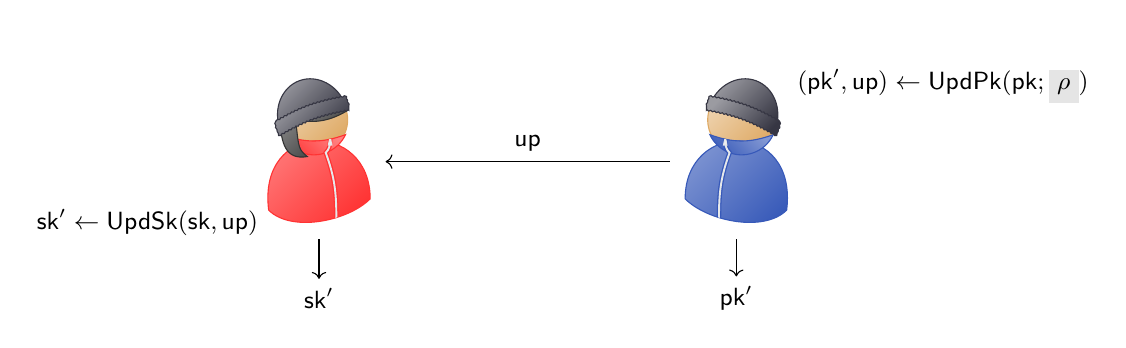
\begin{tikzpicture}[font=\small]
      \node (title) {};
      \node[criminal,female,shirt=red,minimum size=1.3cm, anchor=north west] at ($(title.south east)+(0,-.5)$) (A) {};
      \node[criminal,right=4cm of A,minimum size=1.3cm,mirrored] (B) {};
      \node[anchor=west] at (B.north east) (b1)  {\((\pk', \up) \gets \updpk(\pk; \text{\colorbox{gamechangecolor}{\(\rho\)}})\)};
      \draw (A.0) edge[<-] node[above] {\(\up\)} (B.180);
      \node[anchor=east] at (A.south west) (a2)  {\(\sk' \gets \updsk(\sk, \up)\)};
      \draw (A.270) ++(0,-.75) node {\(\sk'\)} edge[<-] (A.270);
      \draw (B.270) ++(0,-.75) node {\(\pk'\)} edge[<-] (B.270);
    \end{tikzpicture}
  \end{figure}
  \vfill
  \begin{itemize}[label=\textbullet]
    \item Update correctness: Dec. cor. holds for updated keys \((\pk', \sk')\).
  \end{itemize}
\end{frame}

\begin{frame}
  \frametitle{IND-CR-CPA Security Experiment}
  \centering
  \begin{pchstack}[boxed]
    \procedure[mode=text]{$\mathsf{IND}\mhyphen\mathsf{CR}\mhyphen\mathsf{CPA}_{\Pi, \adv}(\secparam)$}{%
      \(i \coloneqq 0\);\quad
      \(b \sample \bin\) \\
      \((\pk_0, \sk_0) \from \kgen(\secparam)\) \\
      \((\state, \msg_0, \msg_1) \from \adv^{\upd\oracle}(\pk_0)\) \\
      \(\ctxt \from \enc(\pk_{i}, \msg_b)\)\\
      \(\state \from \adv^{\upd\oracle}(\ctxt, \state)\) \\
      \(j \coloneqq i\)\\
      \((\pk_{j+1}, \up_{j}) \from \updpk(\pk_{j})\) \\
      \(\sk_{j+1} \from \updsk(\sk_{j}, \up_{j})\) \\
      \(b' \from \adv(\pk_{j+1}, \sk_{j+1}, \up_{j}, \state)\) \\
      \pcreturn \(b = b'\)
    }

    \pchspace

    \procedure[mode=text]{Oracle $\upd\oracle(\rnd)$}{%
      \pclinecomment{Update honestly using} \\
      \pclinecomment{potentially malicious randomness.} \\
      \((\pk_{i+1}, \up_i) \from \updpk(\pk_i; \rnd)\) \\
      \(\sk_{i+1} \from \updsk(\sk_i, \up_i)\) \\
      \(i \coloneqq i + 1\)
    }
  \end{pchstack}
\end{frame}

\begin{frame}
  \frametitle{IND-CR-CPA Security}
  \[
    \left(\pk, \enc(\pk, \msg_0), \pk', \sk', \up\right) \underset{c}{\approx} \left(\pk, \enc(\pk, \msg_1), \pk', \sk', \up\right)
  \]
  \centering \(\implies\) ``forward secrecy.''
\end{frame}

\begin{frame}{Dual-Regev Encryption~\cite{STOC:Regev05,STOC:GenPeiVai08}}
  \begin{figure}
  \begin{pchstack}[boxed]
    \procedure[mode=text]{$\kgen(\secparam)$}{
      \(\mat{A} \sample \ZZ_q^{n \times k}\) \\
      \gamechange{\(\vec{r} \sample \set{\pm 1}^n\)} \\
      \(\vec{u}^\transpose \coloneqq \vec{r}^\transpose \cdot \mat{A} \bmod q\) \\
      \(\pk \coloneqq (\mat{A}, \vec{u})\) \\
      \(\sk \coloneqq \vec{r}\) \\
      \pcreturn \((\pk, \sk)\)
    }

    \pchspace

    \begin{pcvstack}[]
      \procedure[mode=text]{$\enc(\pk,\msg \in \bin)$}{
        \(\vec{x} \sample \ZZ_q^k\);\quad
        \(\vec{e} \sample \chi^n\);\quad
        \(e' \sample \chi\) \\
        \(\vec{c}_0 \coloneqq \mat{A} \cdot \vec{x} + \vec{e} \bmod q\) \\
        \(c_1 \coloneqq \inner{\vec{u}}{\vec{x}} + e' + \round{\frac{q}{2}} \cdot \msg \bmod q\) \\
        \pcreturn \(\ctxt \coloneqq (\vec{c}_0, c_1)\)
      }

      \pcvspace

      \procedure[mode=text]{$\dec(\sk,\ctxt)$}{
        \pcreturn \(\round{\frac{2}{q} \cdot (c_1 - \inner{\vec{r}}{\vec{c}_0} \bmod q)}\)
      }
    \end{pcvstack}
  \end{pchstack}
  \end{figure}
  \vfill
  \begin{itemize}[label=\textbullet]
    \item Correctness: \(\vec{r}\), \(\vec{e}\), \(e'\) are short enough \(\implies\) Dual-Regev has decryption correctness.
      \vfill
    \item Security: LWE assumption \(\implies\) Dual-Regev is IND-CPA secure.
  \end{itemize}
\end{frame}

\begin{frame}{Prior LWE key-update mechanism~\cite{TCC:DodKarWic21}}
  \begin{figure}
    \centering
    \begin{pchstack}[boxed]
      \procedure[mode=text]{$\updpk(\pk)$}{
        \((\mat{A}, \vec{u}) \gets \pk\) \\
        \(\delta \sample \chi_\vec{r}^n\) \\
        \(\pk' \coloneqq (\mat{A}, \vec{u}^\transpose + \delta^\transpose\cdot\mat{A})\) \\
        \(\up \gets \enc(\pk, \delta)\) \\
        \pcreturn \((\pk', \up)\)
      }

      \pchspace

      \procedure[mode=text]{$\updsk(\sk,\up)$}{
        \(\vec{r} \gets \sk\) \\
        \(\delta \gets \dec(\sk, \up)\) \\
        \gamechange{\(\sk' \coloneqq \vec{r} + \delta\)} \\
        \pcreturn \(\sk'\)
      }
    \end{pchstack}
  \end{figure}
  \vfill
  \pause
  \textbf{Issues:}
  \begin{itemize}[label=\textbullet]
    \item Updated secret key \(\vec{r'} = \vec{r} + \delta\) has increased norm.
      \vfill
    \item To maintain correctness with many updates, either 
      \begin{itemize}[label=\textendash]
        \item restrict number of updates to be fixed a-priori, or 
        \item for \(\poly[\secpar]\) many updates, set super-poly. modulus \(q > \secpar^{\omega(1)}\) \(\implies\) large \(\ctxt\).
      \end{itemize}
  \end{itemize}
\end{frame}

\begin{frame}
  \centering
  \textbf{What if we rotate keys instead?}
\end{frame}

\begin{frame}
  \centering
  \visible<1->{
  \textbf{Prior method: Adding noise}
  \begin{tikzpicture}
    \node (a0) at (0,0) {
\includegraphics[scale=0.2]{sk.png}};
    \node (b0) at (3,0) {
\includegraphics[scale=0.2]{sk-blur.png}};
    \node (c0) at (6,0) {\(\cdots\)};
    \node (d0) at (9,0) {
\includegraphics[scale=0.2]{sk-gone.png}};
    \draw (a0) edge[black,thick,->] node[above] {\(+\delta_1\)} (b0);
    \draw (b0) edge[black,thick,->] node[above] {\(+\delta_2\)} (c0);
    \draw (c0) edge[black,thick,->] node[above] {\(+\delta_t\)} (d0);
  \end{tikzpicture}
  }
  \vfill
  \visible<2->{
  \textbf{Our Approach: Rotating keys}
  \begin{tikzpicture}
    \node (a0) at (0,0) {
\includegraphics[scale=0.2]{sk.png}};
    \node (b0) at (3,0) {
\includegraphics[scale=0.2]{sk-rotated1.png}};
    \node (c0) at (6,0) {\(\cdots\)};
    \node (d0) at (9,0) {
\includegraphics[scale=0.2]{sk-rotated2.png}};
    \draw (a0) edge[black,thick,->] node[above] {\(\varphi_1\)} (b0);
    \draw (b0) edge[black,thick,->] node[above] {\(\varphi_2\)} (c0);
    \draw (c0) edge[black,thick,->] node[above] {\(\varphi_t\)} (d0);
  \end{tikzpicture}
  }
\end{frame}

\begin{frame}{$q$-ary Lattices}
  A lattice \(\Lambda \subseteq \RR^n\) is a discrete additive subgroup of \(\RR^n\), i.e. 
      \[
        \Lambda = \mat{B} \cdot \ZZ^{k}
      \]
      for some basis \(\mat{B} \in \RR^{n \times k}\) where \(k \leq n\). All bases \(\mat{B}, \mat{B}' \in \RR^{n \times k}\) are related by unimodular \(\mat{U} \in \ZZ^{k \times k}\) via \(\mat{B}' = \mat{B} \cdot \mat{U}\). 
  \vfill
  Define the Construction A lattice of a full-rank \(\mat{A} \in \ZZ_q^{n \times k}\) as
  \[
    \Lambda_q(\mat{A}) = \mat{A} \cdot \ZZ^k + q \cdot \ZZ^n.
  \] 
  \vfill
  Note that \(\Lambda_q(\mat{A})\) is \(q\)-ary, i.e. 
  \[
    q \cdot \ZZ^n \subseteq \Lambda_q(\mat{A}) \subseteq \ZZ^n.
  \]
\end{frame}

\begin{frame}{LWE and Dual-Regev: Lattice point of view}
  \nonexpert{
  For \(\mat{A} \sample \ZZ_q^{n \times k}\), \(\vec{x} \sample \ZZ_q^k\), short noise \(\vec{e} \sample \chi^n\), consider
  \[
      \text{\bfseries\drawmatrix[height=3,width=.5]b}
      =
      \text{\bfseries\drawmatrix[height=3,width=1.5]A} \;
      \text{\bfseries\drawmatrix[height=1.5,width=.5]x} +
      \text{\bfseries\drawmatrix[height=3,width=.5]e}
      \bmod q.
  \]
  \vfill
  }{}
  LWE assumption: for \(\mat{A} \sample \ZZ_q^{n \times k}\), \(\vec{x} \sample \ZZ_q^k\), \(\vec{e} \sample \chi^n\), \(\vec{u} \sample \ZZ_q^n\) we have \(\left(\mat{A}, \mat{A} \cdot \vec{x} + \vec{e} \bmod q\right) \underset{c}{\approx} \left(\mat{A}, \vec{u} \right)\).

  % Lattice point of view: \(\left(\mat{A},\ \unif{\Lambda_q(\mat{A})} + \chi^n\right) \underset{c}{\approx} \left(\mat{A},\ \unif{\ZZ_q^n}\right).\)
  % \vfill
  \nonexpert{
    Dual-Regev key-pair: \(\left(\mat{A}, \vec{r}^\transpose\cdot\mat{A}\right) \underset{s}{\approx} \left(\mat{A}, \vec{u}^\transpose \sample \ZZ_q^k \right)\) for short \(\vec{r}\) by LHL, or \(\underset{c}{\approx}\) by LWE.
  }{
    A Dual-Regev secret key is a short vector
    \[
      \vec{r} \in \Lambda_q^{\vec{u}}(\mat{A}) \coloneqq \set{ \vec{x} \in \ZZ^n : \vec{x}^\transpose \cdot \mat{A} = \vec{u}^\transpose \bmod q }
    \]
    which is a random lattice coset (defined by \(\vec{u}\)) of the kernel lattice
    \[
      \Lambda_q^{\bot}(\mat{A}) \coloneqq \set{ \vec{x} \in \ZZ^n : \vec{x}^\transpose \cdot \mat{A} = \vec{0}^\transpose \bmod q }.
    \]
  }
\end{frame}

\begin{frame}{Lattice Isomorphism Problem (LIP)}
  \textbf{Lattice Isomorphism:}
    Lattices \(\Lambda, \Lambda'\) are isomorphic, denoted \(\Lambda \sim \Lambda'\),
    if there exists an orthogonal matrix \(\mat{O} \in \Ort_n(\RR)\), i.e. 
    \[
      \mat{O} \in \RR^{n \times n} \qquad\text{with}\qquad \mat{O}^\transpose \cdot \mat{O} = \mat{I}_n,
    \]
    such that 
    \[
      \Lambda' = \mat{O} \cdot \Lambda,
    \]
    i.e. \(\Lambda'\) can be obtained by rotating and reflecting \(\Lambda\). If \(\mat{B}\) and \(\mat{B}'\) are bases of \(\Lambda\) and \(\Lambda'\), then it means \(\mat{B}' = \mat{O} \cdot \mat{B} \cdot \mat{U}\) for some unimodular \(\mat{U} \in \ZZ^{k \times k}\).
  \vfill
  \pause
  \textbf{Lattice Isomorphism Problem (\(\Delta\)LIP)~\cite{EC:DucvWo22}:}
    Given lattices \(\Lambda_0, \Lambda_1, \Lambda \subseteq \RR^n\), decide if
    \[
      \Lambda \sim \Lambda_0 \qquad\text{or}\qquad \Lambda \sim \Lambda_1.
    \]
\end{frame}

\begin{frame}{Rotate Keys with LIP?}
  \textbf{The idea, more concretely:}
  \begin{itemize}[label=\textbullet]
    \item Rotate the lattice: \(\mat{A}\) \(\mapsto\) \(\mat{A}' \coloneqq \mat{O} \cdot \mat{A} \cdot \mat{U} \bmod q\).
    \item Rotate the key: \(\vec{r}\) \(\mapsto\) \(\vec{r}' \coloneqq \mat{O} \cdot \vec{r} \bmod q\).
    \item Update the syndrome: \(\vec{u}\) \(\mapsto\) \(\vec{u}' \coloneqq \mat{U}^\transpose \cdot \vec{u} \bmod q\), so that:
  \end{itemize}
  \vfill
  \[
    \vec{r}^\transpose \cdot \mat{A} = \vec{u}^\transpose
    \qquad
    \implies
    \qquad
    \vec{r'}^\transpose \cdot \mat{A'} = \vec{u'}^\transpose
  \]
  \vfill
  One can think of it as re-randomising a SIS commitment.
  \vfill
  \pause
  \textbf{Upshot:}
  \(\norm{\vec{r'}}_2 = \sqrt{\inner{\mat{O}\cdot\vec{r}}{\mat{O}\cdot\vec{r}}} = \sqrt{\inner{\vec{r}}{\vec{r}}} = \norm{\vec{r}}_2\).
  \vfill
  \pause
  \textbf{Issue:}
  Orthogonal \(\mat{O} \in \Ort_n(\RR)\) are real-valued
  \(\implies\) \(\mat{O} \cdot \mat{A} \cdot \mat{U}\) and \(\mat{O} \cdot \vec{r}\) may not be integral.
\end{frame}

\begin{frame}{Lattice Automorphism of \(\ZZ^n\)}
  \begin{itemize}[label=\textbullet]
    \item The automorphism group \(\Aut(\Lambda)\) of a lattice \(\Lambda\) is the group of all isomorphisms from \(\Lambda\) to itself.
      \vfill
    \item It is well-known that \(\Aut(\ZZ^n) = \Ort_n(\ZZ)\), i.e. the group of signed permutations
      \[
        \Ort_n(\ZZ) = \set{ \mat{D} \cdot \mat{P} \; ; \;  \mat{D} \in \mathsf{diag}(\{\pm 1\}^n),~\mat{P} \in \mathcal{P}_n }.
      \]
      \vfill
      \pause
    \item Since 
      \[
        q \cdot \ZZ^n \subseteq \Lambda_q(\mat{A}) \subseteq \ZZ^n,
      \] 
      we have 
      \[
        q \cdot \ZZ^n \subseteq \mat{O} \cdot \Lambda_q(\mat{A}) = \Lambda_q(\mat{O}\cdot\mat{A}) \subseteq \ZZ^n,
      \]
      i.e. rotating \(\Lambda_q(\mat{A})\) by \(\mat{O} \in \Ort_n(\ZZ)\) gives another \(q\)-ary lattice.
  \end{itemize}
\end{frame}

\begin{frame}{Coding theory point of view}
  \begin{itemize}[label=\textbullet]
    \item The Construction A lattice of \(\mat{A} \in \ZZ_q^{n \times k}\) defined by \(\Lambda_q(\mat{A}) = \mat{A} \cdot \ZZ^k + q \cdot \ZZ^n\) is isomorphic to the \([n,k]\)-linear code \(\code = \mat{A} \cdot \ZZ_q^k\) over \(\ZZ_q\) generated by \(\mat{A}\).
      \vfill
      \pause
    \item The (Signed) Permutation Code Equivalence ((S)PCE) problem is to decide if two codes \(\code\) and \(\code'\) are (signed) permutation equivalent, i.e. whether
      \[
        \code' = \mat{O} \cdot \code
      \]
      for some (signed) permutation matrix \(\mat{O} \in \Ort_n(\ZZ)\).
      \vfill
      \pause
    \item SPCE is essentially decision LIP with \(\Lambda\)'s restricted to \(q\)-ary lattices and \(\mat{O}\)'s restricted to signed permutations.
  \end{itemize}
\end{frame}

\begin{frame}{PCE-based key-update mechanism}
  \begin{figure}
    \centering
    \begin{pchstack}[boxed]
      \procedure[mode=text]{$\updpk(\pk)$}{
        \((\mat{A}, \vec{u}) \gets \pk\) \\
        \(\mat{O} \sample \Ort_n(\ZZ)\) \\
        \(\mat{A'}, \mat{U} \coloneqq \SF(\mat{O}\cdot\mat{A})\) \\
        \(\pk' \coloneqq (\mat{A'}, \vec{u}^\transpose\cdot\mat{U})\) \\
        \(\up \gets \enc(\pk, \mat{O})\) \\
        \pcreturn \((\pk', \up)\)
      }

      \pchspace

      \procedure[mode=text]{$\updsk(\sk,\up)$}{
        \(\vec{r} \gets \sk\) \\
        \(\mat{O} \gets \dec(\sk, \up)\) \\
        \(\sk' \coloneqq \mat{O}\cdot\vec{r}\) \\
        \pcreturn \(\sk'\)
      }
    \end{pchstack}
  \end{figure}
  \vfill
  Update correctness: 
  \[
    \vec{r'}^\transpose \cdot \mat{A'}
    = \vec{r}^\transpose \cdot \underbrace{\mat{O}^\transpose \cdot \mat{O}}_{\mat{I}_n} \cdot \mat{A} \cdot \mat{U}
    = \underbrace{\vec{r}^\transpose \cdot \mat{A}}_{\vec{u}^\transpose} \cdot \mat{U}
    = \vec{u}^\transpose \cdot \mat{U}
    = \vec{u'}^\transpose \pmod q.
  \]
\end{frame}

\begin{frame}{Caution -- Mind the Hull}
  \begin{itemize}[label=\textbullet]
  \item The hardness of (S)PCE, depends on the hull of the code \(\code = \mat{A} \cdot \ZZ_q^k\).
  \item The hull \(\mathcal{H}(\code) \coloneqq \code \cap \code^\bot = \set{ \vec{x} \in \code \; ; \;  \vec{x}^\transpose \cdot \code = \vec{0} }\) is a subcode of \(\code\).
  \item Random codes have small hull dimension~\cite{Sendrier1997}, most likely \(0\).
  \item Existing attacks against (S)PCE run in time \(\bigO{q^h \cdot \poly[n,k]}\) or \(\bigO{n^h \cdot \poly[n,k,q]}\), i.e. efficient when \(h\) is small~\cite{Sendrier2000SSA,BOST2019}.
  \item Up to now, only LCD (\(h=0\)) and self-orthogonal (\(h=k\)) codes have been treated in the literature, and not algorithmically.
  \end{itemize}


  \begin{block}{\(\SampleCode(n,k,h,q)\)}
    We give an algorithm \(\SampleCode(n,k,h,q)\) that samples \(\mat{A}\) generating a uniformly random \([n,k]\)-linear code over \(\ZZ_q\) with hull dimension \(h\). We call such codes and matrices ``\(h\)-hollow''.
  \end{block}
\end{frame}


\begin{frame}
  \frametitle{Sample Self-Dual Vectors}
  \textbf{Definition:} A vector \(\vec{v} \in \code\) is \emph{self-orthogonal} if \(\inner{\vec{v}}{\vec{v}} = 0\).
  \vfill
  \textbf{Observation:} \(\vec{v} = \mat{A}\cdot\vec{x} \in \Span(\mat{A})\) is self-orthogonal iff \(\vec{x}^\transpose\cdot\mat{A}^\transpose\cdot\mat{A}\cdot\vec{x} = 0\).
  \vfill
  Warning's Second Theorem~\cite{ChevalleyWarning1935} implies there are at least \(q^{k-2}\) self-orthogonal vectors in any code.
  \vfill
  \textbf{Algorithm idea:}
  \begin{itemize}[label=\textbullet]
  \item Sample \(\vec{x}_i \sample \ZZ_q\) for \(i=1,\dots,k-2\).
  \item Solve the conic equation \(\vec{x}^\transpose\cdot\mat{A}^\transpose\cdot\mat{A}\cdot\vec{x} = 0\) for \((\vec{x}_{k-1},\vec{x}_k)\).
  \item Complete \(\vec{x}\) with a random solution (and adjust the probability).
  \end{itemize}
\end{frame}


\begin{frame}
  \frametitle{Solving Conics over Finite Fields}
    \textbf{Definition:} A smooth affine conic is an equations of the form
    \[
      A \cdot x^2 + B \cdot xy + C \cdot y^2 + D \cdot x + E \cdot y + F = 0,
    \]
    where \(\Delta = B^2 - 4 \cdot A \cdot C \neq 0\).
  \vfill
   A conic over a finite field \(\FF\) of odd characteristic always has a solution. If \(\Delta \in \QR(\ZZ_q)\) then the number of solutions \(S \in \set{q-1, 2\cdot q - 1}\) and if \(\Delta \notin \QR(\ZZ_q)\) then \(S \in \set{1, q+1}\).
\end{frame}

\begin{frame}
  \frametitle{Adjusting Probabilities with Rejection Sampling}
    Discriminant \(\Delta\) depends on \(\mat{A}\) and is fixed at the beginning of execution. So we know the maximal number of solutions \(M(\Delta)\) is either \(2\cdot q - 1\) or \(q+1\).
  \vfill
    If the conic has \(S\) solutions, we have to accept \(\vec{v}\) with probability \(\frac{S}{M}\), since
    \[
      \prob{\vec{v} = \mat{A}\cdot\vec{x} \text{ sampled}}
      = \frac{1}{q^{k-2}} \cdot \frac{1}{S} \cdot \prob{u \leq \frac{S}{M}}
      = \frac{1}{q^{k-2}} \cdot \frac{1}{M},
    \]
    is then independent of \(S\), hence the distribution is uniform.
\end{frame}

\begin{frame}
  \frametitle{Stealing from the Dual}
    \textbf{Algorithm:}
    \begin{itemize}[label=\textbullet]
      \item Sample a \(0\)-hollow matrix \(\mat{A}_0\) from \(\ZZ_q^{n \times (k-h)}\).
      \item Sample \(\vec{y} \sample \SampleSelfOrthogonal(\Span(\mat{A}_0)^\bot)\) and define \(\mat{A}_1 = [\mat{A}_0, \vec{y}]\).
      \item \dots
      \item Sample \(\vec{y} \sample \SampleSelfOrthogonal(\Span(\mat{A}_{h-1})^\bot)\) and return \(\mat{A}_h = [\mat{A}_{h-1}, \vec{y}] \in \ZZ_q^{n \times k}\).
    \end{itemize}
  \vfill
    The output distribution of this algorithm is negligibly close to the uniform distribution on \([n,k]\)-linear \(h\)-hollow codes over \(\ZZ_q\). It succeeds with prob.
    \[
      \varepsilon \geq \left( 1 - \frac{1}{q} - \frac{1}{q^2} \right) \cdot \left( 1 - \negl[n] \right)
    \]
    if \(2 \cdot k \leq n\) and \(2 \cdot h \leq k\).
\end{frame}

\begin{frame}
  \frametitle{Hollow Lattice Problems}
  \textbf{Upshot:} Now that we know how to sample \(h\)-hollow codes, we can rely on PCE for \(h\)-hollow codes with \(n^h \geq 2^\secpar\) and \(q^h \geq 2^\secpar\) (+ other conditions), which should now be hard.

  \textbf{Question:} Does this somehow make LWE easy?
\end{frame}

\begin{frame}{Hollow Lattice Problems}
    \textbf{Hollow-LWE:} \(\mat{A} \sample \ZZ_q^{n\times k}\) \(h\)-hollow, \(\vec{x} \sample \ZZ_q^k\), \(\vec{e} \sample \chi^n\), \(\vec{u} \sample \ZZ_q^n\), distinguish
    \[
      \left( \mat{A}, \mat{A}\cdot\vec{x}+\vec{e} \right)
      \qquad\text{from}\qquad
      \left( \mat{A}, \vec{u} \right).
    \]
  \vfill
  \begin{theorem}[LWE \(\to\) Hollow-LWE]
    If there exists a \((t,\varepsilon)\)-algorithm \(\adv\) for \(\LWE^h_{k,n,q,\chi}\) then there exists a \((t + \poly, \varepsilon')\)-algorithm \(\bdv\) for \(\LWE_{k-h,n,q,\chi}\) where
    \[
      \epsilon'
      \geq \varepsilon
      \cdot \underbrace{\left( 1-\frac{1}{q}-\frac{1}{q^2} \right)}_\text{triv. hull}
      \cdot \underbrace{\left( 1 - \frac{h}{e^n} \right)}_\text{sub-sampler}
      \cdot \underbrace{\prod_{i=0}^{k-h} \left( 1 - q^{i-n} \right)}_\text{full rank}
      \cdot \underbrace{\prod_{i=1}^{h} \left( 1 - q^{k + i - n} \right)}_\text{lin. dep. in hull}.
    \]
  \end{theorem}
\end{frame}

\begin{frame}{Hollow Lattice Problems}
  \begin{theorem}[Hollow-LHL]
    Let \(n, k, h, q\) integers with
    \[
      n \geq \underbrace{(1+c) \cdot k \cdot \log_2(q)}_\text{LHL} + \underbrace{k + h}_\text{extra}
    \]
    for a positive real constant \(c > 0\), \(h \leq \frac{k}{2}\), and \(q\) an odd prime. Let \(\mat{A} \sample \ZZ_q^{n \times k}\) \(h\)-hollow matrix, \(\vec{r} \sample \set{\pm 1}^n\), and \(\mat{u} \sample \ZZ_q^k\). Then the pairs
    \[
      (\mat{A}, \vec{r}^\transpose \cdot \mat{A}) \qquad \text{and} \qquad (\mat{A}, \vec{u}^\transpose)
    \]
    are statistically close in \(k\).
  \end{theorem}
\end{frame}


\begin{frame}
  \frametitle{Our Construction}
  \centering
  \begin{pchstack}
    \procedure[mode=text]{$\kgen(\secparam)$}{
      \gamechange{\(\mat{A} \sample \SampleCode(n,k,h,q)\)} \\
      \(\vec{r} \sample \set{\pm 1}^n\) \\
      \(\vec{u}^\transpose \coloneqq \vec{r}^\transpose \cdot \mat{A} \bmod q\) \\
      \(\pk \coloneqq (\mat{A}, \vec{u})\) \\
      \(\sk \coloneqq \vec{r}\) \\
      \pcreturn \((\pk, \sk)\)
    }

    \pchspace

    \begin{pcvstack}
      \procedure[mode=text]{$\enc(\pk,\msg \in \ZZ \cap [-p/2, p/2))$}{
        \(\vec{x} \sample \ZZ_q^k\);\quad
        \(\vec{e} \sample \chi^n\);\quad
        \(e' \sample \chi\) \\
        \(\vec{c}_0 \coloneqq \mat{A} \cdot \vec{x} + \vec{e} \bmod q\) \\
        \(c_1 \coloneqq \inner{\vec{u}}{\vec{x}} + e' + \round{\frac{q}{p}} \cdot \msg \bmod q\) \\
        \pcreturn \(\ctxt \coloneqq (\vec{c}_0, c_1)\)
      }

      \pcvspace

      \procedure[mode=text]{$\dec(\sk,\ctxt)$}{
        \pcreturn \(\round{\frac{p}{q} \cdot (c_1 - \inner{\vec{r}}{\vec{c}_0} \bmod q)}\)
      }
    \end{pcvstack}

    \pchspace

    \procedure[mode=text]{$\updpk(\pk)$}{
      \(\rho \sample \bin^\secpar\) \\
      \(\mat{O} \coloneqq \hash(\rho)\) \\
      \((\mat{A}', \mat{U}) \coloneqq \SF(\mat{O}\cdot \mat{A})\)\\
      \({\vec{u}'}^\transpose \coloneqq  \vec{u}^\transpose \cdot \mat{U} \bmod q\) \\
      \(\pk' \coloneqq (\mat{A}', \vec{u}')\) \\
      \(\up \gets \enc(\pk, \rho)\) \\
      \pcreturn \((\pk', \up)\)
    }

    \pchspace

    \procedure[mode=text]{$\updsk(\sk,\up)$}{
      \(\rho \gets \dec(\sk,\up)\) \\
      \(\mat{O} \coloneqq \hash(\rho)\) \\
      \(\vec{r}' \coloneqq \mat{O} \cdot \vec{r}\) \\
      \pcreturn \(\sk' \coloneqq \vec{r'}\)
    }
  \end{pchstack}
\end{frame}

\begin{frame}
  \frametitle{Security Theorem}

  Our construction is the Dual-Regev PKE with
  \begin{itemize}[label=\textbullet]
    \item \(\mat{A} \sample \SampleCode(n,k,h,q)\),
    \item \(\vec{r} \sample \set{\pm 1}^n\), and
    \item the above PCE-based update mechanism.
  \end{itemize}

  \begin{theorem}
    Let \(n, k, h, q\) be positive integers parametrised by \(\secpar\) with \(n \geq (1 + c) \cdot k \cdot \log_2(q) + k + h\) for a positive real constant \(c>0\), \(2 \cdot h \leq k\) and \(q\) prime.

    Assuming the advantage of any \(\ppt\) adversary in distinguishing \(\LWE_{k,n,q,\chi}^h\) and in distinguishing \(\PCE_{n,k,q}^h\) is negligible in \(\secpar\), our construction is IND-CR-CPA secure in the ROM.
  \end{theorem}

\end{frame}

\begin{frame}
  \frametitle{\(\text{Game}_4 \overset{?}{\approx} \text{Game}_5\)}

  \begin{columns}

    \begin{column}{0.5\linewidth}
      \begin{align*}
        \pk_0 &= (\mat{A},\vec{u}),\\
        \pk &= (\mat{O}\cdot\mat{A}\cdot\mat{U},\ \mat{U}^\transpose\cdot\vec{u}),\\
        \sk &= \mat{O}\cdot\vec{r},\\
        \ctxt &\from \enc((\mat{A},\vec{u}), \msg_b),\\
        \up &= \enc((\mat{A},\vec{u}),\rnd^*); \\
        \\
        \vec{r} &\sample \set{\pm 1}^n,\\
        \vec{u}^\transpose &= \vec{r}^\transpose \cdot \mat{A},\\
        \mat{O} & \sample \Ort_n(\ZZ)
      \end{align*}
    \end{column}
    \begin{column}{0.5\linewidth}
      \begin{align*}
        \pk_0 &= (\mat{A},\vec{u}),\\
        \pk &= \gamechange{(\mat{B},\vec{v})},\\
        \sk &= \gamechange{\vec{r}'},\\
        \ctxt &\from \enc((\mat{A},\vec{u}), \msg_b),\\
        \up &= \enc((\mat{A},\vec{u}),\rnd^*); \\
        \\
        \vec{r},\vec{r}' &\sample \set{\pm 1}^n,\\
        \vec{u}^\transpose &= \vec{r}^\transpose \cdot \mat{A},\\
        \vec{v}^\transpose &= \vec{r}'^\transpose\cdot\mat{B}
      \end{align*}
    \end{column}
  \end{columns}
\end{frame}

\begin{frame}
  \frametitle{\(\text{Game}_4 \approx \text{Game}_5\): The stars just about align}
  \begin{itemize}[label=\textbullet]
    \item<1-> Take a \(h\)-hollow PCE instance \((\mat{A}, \mat{B})\). Compute \(\vec{a}^\transpose = \sum_{i=1}^{n} \mat{A}_i\) and \(\mat{b}^\transpose = \sum_{i=1}^{n} \mat{B}_i\). Then \([1]^n\) is a valid secret for \((\mat{A},\vec{a})\) and \((\mat{B},\vec{b})\).
      \vfill
    \item<2-> Sample \(\mat{O}_\mat{A}, \mat{O}_\mat{B} \sample \Ort_n(\ZZ)\), \(\mat{U}_\mat{A}, \mat{U}_\mat{B} \sample \GL_k(\ZZ_q)\), and compute
      \begin{align*}
        \mat{A'} &= \mat{O}_\mat{A}\cdot\mat{A}\cdot\mat{U}_\mat{A} &\vec{a'}^\transpose &= \vec{a}^\transpose\cdot\mat{U}_\mat{A} &\vec{r}_\mat{A} &= \mat{O}_\mat{A}\cdot [1]^n \\
        \mat{B'} &= \mat{O}_\mat{B}\cdot\mat{B}\cdot\mat{U}_\mat{B} &\vec{b'}^\transpose &= \vec{b}^\transpose\cdot\mat{U}_\mat{B} &\vec{r}_\mat{B} &= \mat{O}_\mat{B}\cdot [1]^n
      \end{align*}
      \vfill
    \item<3-> If \(\mat{B} = \SF(\mat{P}\cdot\mat{A})\), then \(\mat{O}_\mat{B}\cdot\mat{P}\cdot\mat{O}_\mat{A}^{-1}\) updates \(((\mat{A'}, \vec{a'}), \vec{r}_\mat{A})\) to \(((\mat{B'}, \vec{b'}), \vec{r}_\mat{B})\), since for any \(\mat{P}\) we have \([1]^n = \mat{P}\cdot [1]^n\), otherwise random.
      \vfill
    \item<4-> Thus any distinguisher \(\ddv_{4,5}\) also distinguishes PCE.
  \end{itemize}
\end{frame}


\begin{frame}{Some Parameters and Sizes}
  \begin{table}[htb]
    \centering
    \caption{\textbf{Table 1:} Parameters for the given \(\secpar\) and \(p\) with \(c=0.25\) and \(s = 8\).}\label{tab:params}
    \vspace{0.3\baselineskip}
    \begin{tabular}{l @{\hskip 1em} l @{\hskip 1em} r @{\hskip 1em} r r @{\hskip 1em} r @{\hskip 1em} r @{\hskip 1em} r}
      \toprule
      \(\secpar\) & \(p\) & \(n\) & \(k\) & \(\log_2(q)\) & \(h\) & \(\lvert \ctxt \rvert\) & \(\lvert \up \rvert\) \\
      \midrule
      \(128\) &  \(2\) & \(7313\)  &  \(450\) & \(13\) & \(27\) & \(11.6\) KiB & \(1485.7\) KiB\\
      \(128\) & \(16\) & \(11000\) &  \(550\) & \(16\) & \(26\) & \(21.5\) KiB &  \(687.6\) KiB\\
      \(192\) & \(32\) & \(20250\) &  \(900\) & \(18\) & \(37\) & \(44.5\) KiB & \(1708.7\) KiB\\
      \(256\) & \(32\) & \(29688\) & \(1250\) & \(19\) & \(48\) & \(68.9\) KiB & \(3525.6\) KiB\\
      \midrule
      \multicolumn{8}{c}{\cite{AC:HaiPasSte23} with \(2^{20}\) updates}\\
      \midrule
      \(128\) &     -- &        -- &       -- & \(36\) &     -- &  \(9.1\) KiB &     \(27\) KiB \\
      \bottomrule
    \end{tabular}
  \end{table}
\end{frame}

\begin{frame}
  \frametitle{Future Work}
  \begin{itemize}[label=\textbullet]
    \item Replace the Hollow LHL with a computational assumption.
    \item Switch from LWE to MLWE.
    \item Consider the model from~\cite{EC:AlwFucMul24}.
    \item \dots
  \end{itemize}
\end{frame}

\begin{frame}
  \centering
  Thank you! Read the full version at \href{https://eprint.iacr.org/2025/340}{\underline{ia.cr/2025/340}}:

  
\includegraphics[]{qr.png}
\end{frame}

\begin{frame}[allowframebreaks]
  \frametitle{Bibliography}

  \bibliographystyle{alpha}
  \bibliography{abbrev3,crypto,local}

\end{frame}


\end{document}

%%% Local Variables:
%%% mode: LaTeX
%%% TeX-master: t
%%% End:
